\chapter{Introduction}
\label{chap:introduction}

\section{Citation styles}

These are the different citation styles for author-year.

The standard \verb=\cite= command produces the following output: \cite{clarke1990rendezvous}.

The \verb=\textcite= command produces the following output: \textcite{clarke1990rendezvous}.

\clearpage          % To start a new page

\section{Figures}

Always prefer to float figures to the top of the page using the [t] option in the figure environment.

\begin{figure}[t]
    \centering
    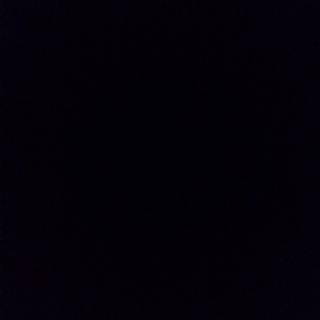
\includegraphics{figures/blackbox.jpeg}
    \caption{This is a black box}
    \label{fig:fig_1}
\end{figure}

\clearpage

\section{Tables}

Use vertical lines sparingly in tables. They're unnecessary bloat. Write the code for tables in a separate tex file, and include it in when required. Also preferrably use sans serif font for tables (because of their information density) using \texttt{\\sffamily} in table definition.

\begin{table}[!ht]
\small
\centering
\sffamily
\begin{tabular}{lccc}
	\toprule
    \textbf{Spam} & \textbf{Ni} & \textbf{Swallow} & \textbf{Shrubbery} \\
    \midrule
    A & 1 & 2 & 3 \\
    \midrule
    E & 3 & 4 & 5 \\
    C & 6 & 9 & 3 \\
    \midrule
    M & 4 & 1 & 1 \\
    \bottomrule
\end{tabular}
\caption{This is a table}
\label{tab:table}
\vspace{-5mm}
\end{table}

